\section{TET Features}
The TET we build a the tree will be rooted in a user U.
U is a user-node in the graph if $User(U) = True$. 

The feature User are in the boolean domain meaning that this feature will be either true false.
\begin{equation}
User(U)\rightarrow \{True, False\}
\end{equation}

Rating is a feature in the domain of low mid or high the original rating have been split into these three categories.
the original ratings went from 0 to 5, where $low<2.5<=mid<=3.5<high$.

\begin{equation}
Rating(U, M) \rightarrow \{Low, Mid, High\}
\end{equation}

Genre is in the domain of movie genes. this feature will return a boolian value when given a muvie m and a genre g, returning true if m are categorised as genre G.
\begin{equation}
Genre(M) \rightarrow \{True, False\}
\end{equation}


The TETs constructed form the DATASET will be build from this structure.
\begin{equation}
User(U) \stackrel{M}{\longrightarrow} Rating(U,M) \longrightarrow Genre(M)
\end{equation}

The TET will represent a neighbourhood of the graph with a User as the root

the sub-trees are them self TETs
\begin{equation}
Rating(U,M) \longrightarrow Genre(M)
\end{equation}

All of these functions has a been intended to work as if they were programmed in a logical paradigm. 

With the functions that can give a boolean result such as User(U) or any of the genres for example Action(M,G) we are only interested in True values. the tree will thefore have a end up having this form

\begin{figure}[H]
    \centering
    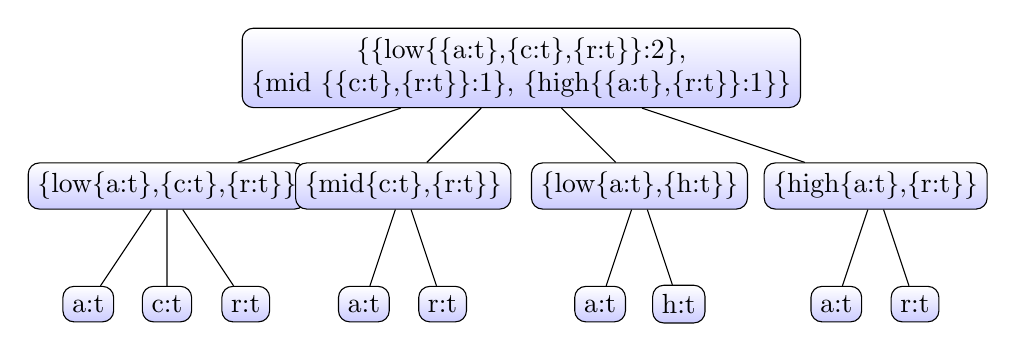
\begin{tikzpicture}[
  	every node/.style = {shape=rectangle, rounded corners,
    draw, align=center,
    top color=white, bottom color=blue!20},
    level 1/.style={sibling distance=3cm},
	level 2/.style={sibling distance=1cm}, 
    ]
  
  \node {\{\{low\{\{a:t\},\{c:t\},\{r:t\}\}:2\},\\
   \{mid \{\{c:t\},\{r:t\}\}:1\}, \{high\{\{a:t\},\{r:t\}\}:1\}\}}
	child{ node{\{low\{a:t\},\{c:t\},\{r:t\}\}} 
		child{ node{a:t}}
		child{ node{c:t}}
		child{ node{r:t}}
		}
	child{ node{\{mid\{c:t\},\{r:t\}\}} 
		child{ node{a:t}}
		child{ node{r:t}}
		}
	child{ node{\{low\{a:t\},\{h:t\}\}} 
		child{ node{a:t}}
		child{ node{h:t}}
		}
    child{ node{\{high\{a:t\},\{r:t\}\}}
	    child { node{a:t}}
      	child { node{r:t}} 
      	}
      ;
\end{tikzpicture}

%
%
%
    \caption{caption}
    \label{fig:caption}
	
\end{figure}

\todo{billedet skal være bedre}

The value of a TET T(X) for a user U will be denoted as V(T(U)). If the node U is not a user or is not part of domain, the value for the tree default to false.\todo{this part has to be more precise and telling look at bottom of p.39 in tet article}

The tree can also be represented as 

\begin{equation}
    T(U)=
    \begin{cases}
      (low \{(action:t),(casual:t)... (romance:t)\}):2 \\
      (low \{(action:t),(horror:t)\}):1 \\
      (mid \{(comedy:t),(romance:t)\}):4 \\
      (high\{(adventure:t),(romance:t)\}):2
    \end{cases}
\end{equation}

This tells that the tree T(U) has 2 movies whith low rating and the genres action, casual, and romance.